\documentclass[UTF8]{ctexart}
\usepackage[a4paper]{geometry} % 调整纸张大小和页边距的包,中括号中规定了纸张大小
\geometry{left=2.0cm,right=2.0cm,top=2.0cm,bottom=2.0cm} % 页边距设置
\usepackage{fancyhdr}
\usepackage{graphicx}
\graphicspath{{figures/}}
% Copyright 20120 Liutao Tian, MIT License
% https://github.com/andy123t/code-latex-style/

\usepackage{listings,color}

% Matlab highlight color settings
%\definecolor{mBasic}{RGB}{248,248,242}       % default
\definecolor{mKeyword}{RGB}{0,0,255}          % bule
\definecolor{mString}{RGB}{160,32,240}        % purple
\definecolor{mComment}{RGB}{34,139,34}        % green
\definecolor{mBackground}{RGB}{245,245,245}   % lightgrey
\definecolor{mNumber}{RGB}{134,145,148}       % gray

\definecolor{Numberbg}{RGB}{237,240,241}     % lightgrey

% Python highlight color settings
%\definecolor{pBasic}{RGB}{248, 248, 242}     % default
\definecolor{pKeyword}{RGB}{228,0,128}        % magenta
\definecolor{pString}{RGB}{148,0,209}         % purple
\definecolor{pComment}{RGB}{117,113,94}       % gray
\definecolor{pIdentifier}{RGB}{166, 226, 46}  %
\definecolor{pBackground}{RGB}{245,245,245}   % lightgrey
\definecolor{pNumber}{RGB}{134,145,148}       % gray

\lstnewenvironment{Python}[1]{
	\lstset{language=python,               % choose the language of the code
		xleftmargin=30pt,
		xrightmargin=10pt,
		frame=l,
		framesep=15pt,%framerule=0pt,  % sets the frame style
		%frame=shadowbox,rulesepcolor=\color{red!20!green!20!blue!20},
		%basicstyle=\small\ttfamily,          % sets font style for the code
		basicstyle=\footnotesize\fontspec{Consolas},
		keywordstyle=\color{pKeyword},       % sets color for keywords
		stringstyle=\color{pString},         % sets color for strings
		commentstyle=\color{pComment},       % sets color for comments
		backgroundcolor=\color{pBackground}, % choose the background color
		title=#1,                            %\lstname show the filename of files
		emph={format_string,eff_ana_bf,permute,eff_ana_btr},
		emphstyle=\color{pIdentifier}
		showspaces=false,                    % show spaces adding particular underscores
		showstringspaces=false,              % underline spaces within strings
		showtabs=false,                      % show tabs within strings adding particular underscores
		tabsize=4,                           % sets default tabsize to 2 spaces
		captionpos=t,                        % sets the caption-position to bottom
		breaklines=true,                     % sets automatic line breaking
		framexleftmargin=5pt,
		fillcolor=\color{Numberbg},
		rulecolor=\color{Numberbg},
		numberstyle=\tiny\color{pNumber},
		numbersep=9pt,                      % how far the line-numbers are from the code
		numbers=left,                        % where to put the line-numbers
		stepnumber=1,                        % the step between two line-numbers.
}}{}

\lstnewenvironment{Python1}[1]{
\lstset{language=python,               % choose the language of the code
  xleftmargin=30pt,
  xrightmargin=10pt,
  frame=l,
  framesep=15pt,%framerule=0pt,  % sets the frame style
  %frame=shadowbox,rulesepcolor=\color{red!20!green!20!blue!20},
  %basicstyle=\small\ttfamily,          % sets font style for the code
  basicstyle=\footnotesize\fontspec{Consolas},
  keywordstyle=\color{pKeyword},       % sets color for keywords
  stringstyle=\color{pString},         % sets color for strings
  commentstyle=\color{pComment},       % sets color for comments
  backgroundcolor=\color{pBackground}, % choose the background color
  title=#1,                            %\lstname show the filename of files
  emph={format_string,eff_ana_bf,permute,eff_ana_btr},
  emphstyle=\color{pIdentifier}
  showspaces=false,                    % show spaces adding particular underscores
  showstringspaces=false,              % underline spaces within strings
  showtabs=false,                      % show tabs within strings adding particular underscores
  tabsize=4,                           % sets default tabsize to 2 spaces
  captionpos=t,                        % sets the caption-position to bottom
  breaklines=true,                     % sets automatic line breaking
  framexleftmargin=5pt,
  fillcolor=\color{Numberbg},
  rulecolor=\color{Numberbg},
  numberstyle=\tiny\color{pNumber},
  numbersep=9pt,                      % how far the line-numbers are from the code
  numbers=left,                        % where to put the line-numbers
  stepnumber=1,                        % the step between two line-numbers.
}}{}



\usepackage{float}
%\usepackage{tocloft}
\pagestyle{fancy}
\begin{document}
	\begin{titlepage}
		\heiti
		\vspace*{64pt}
		\begin{center}
			\fontsize{42pt}{0}{嵌\quad 入\quad 式\quad 系\quad 统\quad 应\quad 用 \quad 项\quad 目}\\
			\vspace*{48pt}
			
			\LARGE 题目:\ \ \underline{\makebox[350pt]{基于STM32F4单片机手写数字识别系统}}\\
			\vspace*{48pt}
			\Large 姓\qquad 名:\ \ \underline{\makebox[108pt]{谢唯嘉}}\ \ \\
			\vspace*{48pt}
			\Large 学\qquad 号:\ \ \underline{\makebox[108pt]{6120210299}}\\
			\vspace*{48pt}
			\Large 指导老师:\ \  \underline{\makebox[108pt]{吴君钦}}\\
		\end{center}
	\end{titlepage}

	\newpage
	\fancyhf{}
	\fancyhead[C]{嵌入式课程设计论文}
	%\setlength{\cftbeforetoctitleskip}{20pt}
	\renewcommand{\contentsname}{\LARGE 目\quad 录}
	\tableofcontents
	\newpage

\section{项目应用背景及意义}
\subsection{项目应用背景}
手写数字识别(Handwritter Numeral Recognition)是光学字符识别技术(Optical Character Recognition,简称OCR)的一个分支,它研究的对象是:如何利用电子计算机自动辨别人手写在电子屏幕上的阿拉伯数字。

OCR是模式识别的一个分支,按字体分类主要分为印刷体识别和手写体识别两大类,而手写体识别又可分为受限手写体和不受限识别体,按识别方式有分为在线识别和脱机识别。在整个OCR领域中,最为困难的就是脱机手写字符的识别。到目前为止,尽管人们在脱机手写英文,汉字识别的研究中已取得很多可喜可贺的成就,但距实用还有一定的距离。而在手写数字识别这个方向上,经过多年研究,研究者已经开始把它向各种实际应用推广,为手写数据的高速自动输入提供了一种解决方案。

手写识别,是指对在手写设备上书写时产生的有序轨迹信息进行识别的过程,是人际交互最自然、最方便的手段之一。随着智能手机和平板电脑等移动设备的普及,手写识别的应用也被越来越多的设备采用。

手写识别能够使用户按照最自然、最方便的输入方式进行文字输入,易学易用,可取代键盘或者鼠标。用于手写输入的设备有许多种,比如电磁感应手写板、压感式手写板、触摸屏、触控板、超声波笔等。

字符识别处理的信息可分为两大类:一类是文字信息,处理的主要是用各国家,各民族的文字书写或印刷的文字信息,目前在印刷体和联机手写方面技术已趋于成熟,并推出了很多应用系统;另一类是数据信息,主要是由阿拉伯数字及少量特殊符号组成的各种编号和统计数据,如:邮政编码,统计报表,财务报表,银行票据等等,处理这类信息的核心技术是手写数字识别。因此,手写数字的识别研究有着重大的现实意义,一旦研究成功并投入应用,将产生巨大的社会和经济效益。
\subsection{项目设计意义}
手写数字识别作为模式识别领域的一个重要问题,也有着重要的理论价值:

1.阿拉伯数字是唯一的被世界各国通用的符号,对手写数字识别的研究基本上与文化无关,这样就为各国,各地区的研究者提供了一个大舞台。在这一领域中大家可以探讨,比较各种研究方法。

2.由于数字识别的类别数较小,有助于做深入分析及验证一些新的理论。

3.尽管人们对手写数字的识别已从事了很长时间的研究,并已取得了很多成果,但到目前为止机器的识别本领还无法与人的认知能力相比,这仍是一个有难度的开放问题

4.手写数字的识别方法很容易推广到其他一些相关问题,很多学者就是把数字和英文字母的识别放在一块研究的。
\section{项目概要设计与功能分析}
\subsection{项目概要设计}
\subsubsection{系统构成}
该手写数字识别系统在大体上可以分为一下几个部分:LED指示灯DS0(连接在PF9),串口1(波特率:115200,PA9/PA10连接在板载USB转串口芯片CH340上面),ALIENTEK 2.8/3.5/4.3/7寸TFTLCD模块(通过FSMC驱动,FSMC\_NE4接LCD片选/A6接RS),按键KEY0(PE4)/KEY2(PE2),W25Q128(SPI FLASH芯片,连接在SPI1上)。STM32F4单片机作为整个手写数字识别系统最重要的模块,它的主要功能是读取显示屏上所采集到的实时数据并进行相应的处理,而后将处理结果通过显示屏显示,再通过SPI传输总线将信号进行传输。​ SPI总线:一种全双工同步串行总线,是微处理控制单元(MCU)和外围设备之间进行通信的同步串行端口。主要应用在EEPROM、Flash、实时时钟(RTC)、数模转换器(ADC)、网络控制器、MCU、数字信号处理器(DSP)以及数字信号解码器之间。电源部分采用USB数据线连接电脑给整个系统供电。如2-1为该手写数字识别系统的设计框图。
\begin{figure}[h]
	\centering
	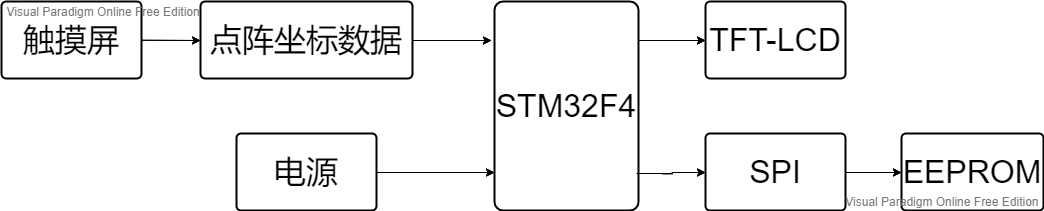
\includegraphics[scale = 0.4]{2}
	\caption{整体系统框图}
\end{figure}
\subsubsection{软件介绍}
Keil软件是德国Keil Software公司推出的软件开发系统,是目前最为流行的80C51系列单片机软件。支持C语言和汇编语言的程序设计,提供了包括C编译器、宏汇编、连接器、库管理和仿真调试器等完整的开发方案,通过一个集成开发环境(u Vision)组合在一起,功能非常强大且方便易用。对于初学者而言,使用Keil软件程序并进行调试时,可以很方便从窗口查看到调试程序时单片机寄存器和存储器的使用、变化情况,有助于修改程序,并模拟分析运行。如图\ref{a}所示为Keil软件的运行界面。

\begin{figure}[h]
	\centering
	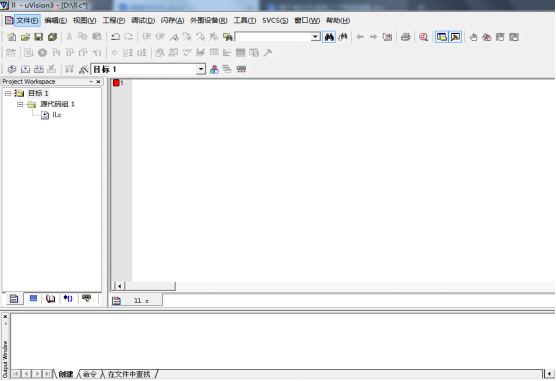
\includegraphics[scale = 0.8]{1}
	\caption{Keil软件运行界面}
	\label{a}
\end{figure}
\subsubsection{SPI接口介绍}
SPI 是英语 Serial Peripheral interface的缩写,顾名思义就是串行外围设备接口。是Motorola首先在其MC68HCXX 系列处理器上定义的。SPI 接口主要应用在 EEPROM,FLASH,实时时钟,AD 转换器,还有数字信号处理器和数字信号解码器之间。SPI,是一种高速的,全双工,同步的通信总线,并且在芯片的管脚上只占用四根线,节约了芯片的管脚,同时为PCB的布局上节省空间,提供方便,正是出于这种简单易用的特性,现在越来越多的芯片集成了这种通信协议,STM32F4 也有 SPI 接口。下面我们看看 SPI 的内部简明图\ref{b}
\begin{figure}[h]
	\centering
	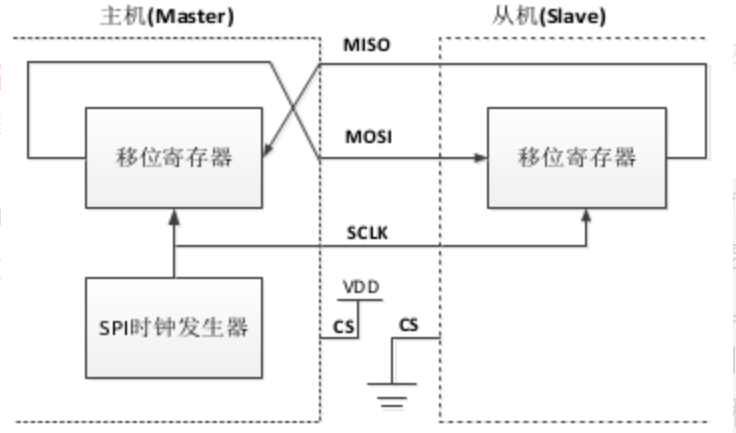
\includegraphics[scale = 0.5]{3}
	\caption{SPI内部简明图}
	\label{b}
\end{figure}
SPI 接口一般使用 4 条线通信:MISO 主设备数据输入,从设备数据输出。MOSI 主设备数据输出,从设备数据输入。SCLK 时钟信号,由主设备产生。CS 从设备片选信号,由主设备控制。

从图中可以看出,主机和从机都有一个串行移位寄存器,主机通过向它的 SPI 串行寄存器写入一个字节来发起一次传输。寄存器通过 MOSI 信号线将字节传送给从机,从机也将自己的移位寄存器中的内容通过 MISO 信号线返回给主机。这样,两个移位寄存器中的内容就被交换。

外设的写操作和读操作是同步完成的。如果只进行写操作,主机只需忽略接收到的字节;反之,若主机要读取从机的一个字节,就必须发送一个空字节来引发从机的传输。

SPI 主要特点有:可以同时发出和接收串行数据;可以当作主机或从机工作;提供频率可编程时钟;发送结束中断标志;写冲突保护;总线竞争保护等。

SPI 总线四种工作方式 SPI 模块为了和外设进行数据交换,根据外设工作要求,其输出串行同步时钟极性和相位可以进行配置,时钟极性(CPOL)对传输协议没有重大的影响。如果CPOL=0,串行同步时钟的空闲状态为低电平;如果 CPOL=1,串行同步时钟的空闲状态为高电平。时钟相位(CPHA)能够配置用于选择两种不同的传输协议之一进行数据传输。如果CPHA=0,在串行同步时钟的第一个跳变沿(上升或下降)数据被采样;如果 CPHA=1,在串行同步时钟的第二个跳变沿(上升或下降)数据被采样。SPI 主模块和与之通信的外设备时钟相位和极性应该一致。
不同时钟相位下的总线数据传输时序如图\ref{c}所示:
\begin{figure}[h]
	\centering
	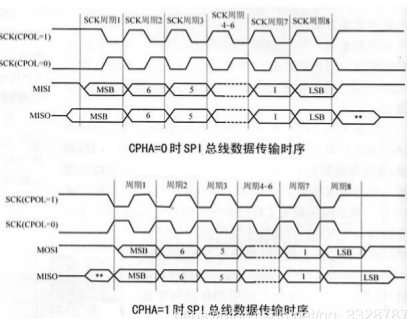
\includegraphics[scale = 0.65]{4}
	\caption{总线数据传输时序}
	\label{c}
\end{figure}
\subsubsection{EEPROM带电可擦可编程只读存储器}
EEPROM (Electrically Erasable Programmable read only memory)是指带电可擦可编程只读存储器。是一种掉电后数据不丢失的存储芯片。如\ref{d}所示, EEPROM 可以在电脑上或专用设备上擦除已有信息,重新编程。

本设计采用EEPROM存储器,旨在将所测得的当前光强信息通过I2C数据传输线存储在EEPROM中,以保证检测并存储一天整光强信息功能的实现。

\begin{figure}[h]
	\centering
	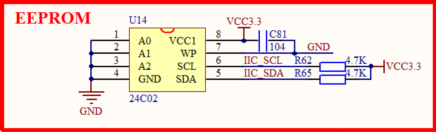
\includegraphics[scale = 0.9]{5}
	\caption{EEPROM带电可擦可编程只读存储器}
	\label{d}
\end{figure}
\subsection{项目功能分析}
本项目是基于STM32F4单片机实时手写数字识别系统,该系统采用STM32F4单片机作为中心处理模块,对所采集到的信息进行加工处理和分析,同时还采用TFT-LCD液晶显示屏、ADC模/数转换模块和 SPI数据传输模块等,实现了对实时液晶显示屏上的手写输入进行动态的采集、处理、显示以及存储20个的手写数字信息,达到了能检测记录不同数字输入的数字识别、显示数字识别信息以及存储的目的。
\section{项目功能部件介绍}
\subsection{TFTLCD模块}
以2.8寸的TFTLCD为例,采用16位的并方式与外界进行连接,模块接口图\ref{e}所示,具有如下一些信号线:

CS:TFTLCD片选信号

WR:向TFTLCD写入数据

RD:从TFTLCD读取数据

D[15:0]:16位双向数据线

RST:硬复位TFTLCD,直接连接到stm32的复位引脚上

RS:命令/数据标志(0,读写命令;1,读写数据)
\begin{figure}[h]
	\centering
	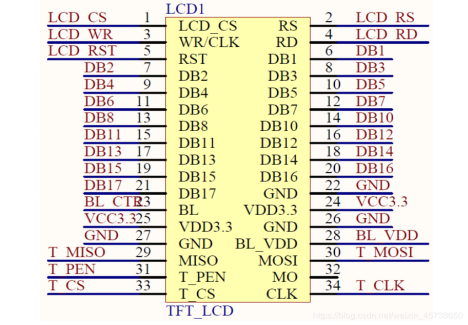
\includegraphics[scale = 0.6]{6}
	\caption{TFTLCD模块接口图}
	\label{e}
\end{figure}
\subsection{ILI9341控制器}
ILI9341控制器是TFTLCD的驱动芯片,在16位的模式下,ILI9341采用RGB565格式储存颜色数据,下面为16位数据与显存的对应关系,最低5位代表蓝色,中间六位代表绿色,最高5位代表红色,数值越大,颜色越深。另外,ILI9341的所有指令都是8位的(高8位无效),并且参数除了读/写GRAM的时候是16位的,其它操作参数都是8位的。

TFTLCD模块的使用流程如图\ref{f}所示
\begin{figure}[h]
	\centering
	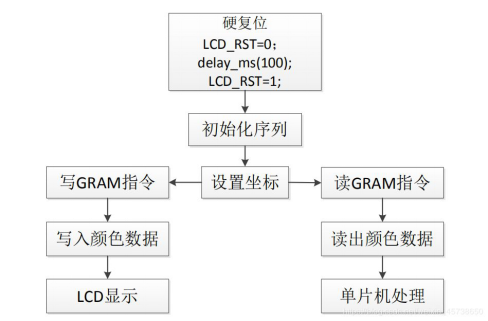
\includegraphics[scale = 0.6]{7}
	\caption{TFTLCD模块工作流程}
	\label{f}
\end{figure}

使用TFTLCD显示字符和数字的过程:首先,设置STM32F1与TFTLCD模块相连接的I/O,用到的是FSMC。然后,初始化TFTLCD模块,最后,通过函数将字符和数字显示到TFTLCD模块上,通过\ref{f}左侧的流程,这只是一个点的处理,要显示字符和数字,就要多次使用这个步骤。

\subsection{OLED液晶显示屏}
本设计用OLED来显示当前的光照强度、温度值和补偿光照强度,使人们能直观地了解到当前的环境状况以及电路工作状况。以便作出更准确的调节,采用的是寸的OLED液晶显示模块,体积小、成本低、功耗低、使用寿命长。可切换界面设计使状态值和调试值分开,简洁易懂。

\section{项目整体硬件电路设计}
\subsection{电源电路分析}
本设计采用交流供电,电源插座部分用的是贴片式DC005,便于手工做板和加工,同时贴片无孔设计可很好的保护介质基板的板结构,使其更加牢固不易损坏,也使供电时相对方便。开关部分并没有采用常用的六脚自锁开关,而是采用了贴片两脚自锁开关,这种开关的优势在于贴片设计,便于加工以及保护基板性能,也便于按键的更换,同时大封装的设计,使电路可以过更大的电流,避免了六角自锁开关因为电流不够而烧坏的危险,使LED充分发光。

电源电路中还有两个稳压模块,一是lm7805,作用是将变压器电源的输入9V电压稳定到5V给整个电路系统供电。三端稳压IC用lm78系列芯片来组成,稳压电源电路内部有多种保护电路,包括过流、过热保护以及调整管,因此使用起来可靠、方便,而且其价格便宜,性价比高,便于商品化批量生产。

\begin{figure}[h]
	\centering
	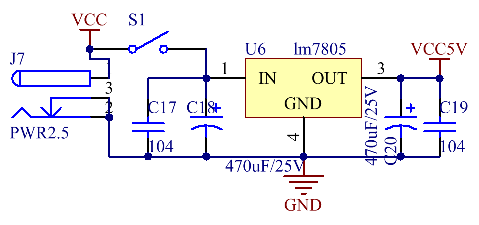
\includegraphics[scale = 0.7]{9}
	\caption{lm7805电源电路}
\end{figure}
还有一个则是AMS1117稳压器,目的是给单片机以及几个外设模块提供稳定的电压。在应用这两个模块时分别用优质钽电容和0805瓷片电容进行了电源滤波,一大一小的电容容量处理,可以使电路中的高频和低频杂波干扰信号充分被吸收,使电路更加稳定可靠。之所以本设计不考虑采用220V供电,以及采用220V的电灯,因为220V已经远远超出了对人体安全的电压范围,容易产生事故,发生危险,同时,5V的LED亮度已经完全能够达到照明效果,且更加节能安全环保。
\begin{figure}[h]
	\centering
	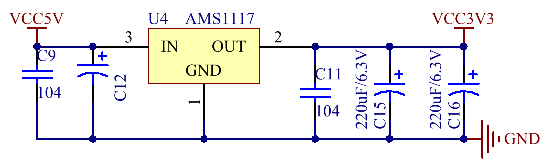
\includegraphics[scale = 0.7]{8}
	\caption{AMS1117电源电路}
\end{figure}
\subsection{USB接口分析}
调试硬件接口硬件电路所示当电脑主机的USB接口接入STMF4设备时,通过USB接口的5V供电电压为USB设备供电;设备得到供电后,内部电路开始工作,并向USB接口的+DATA针脚输出高电平信号(-DATA针脚仍为低电平),同时主板南桥芯片中的USB模块会不停的检测USB接口的+DATE针脚和-DATA针脚的电压,当南桥芯片中的USB模块检测到USB接口的+DATE针脚的高电平信号和-DATA针脚的低电平信号后,就认为USB设备准备好,并向USB设备发出准备好信号,接着设备的控制芯片就通过USB接口向电脑主板的USB总线发送设备的数据信息,电脑主板接收到数据信息后,操作系统就会提示发现新硬件,并开始安装USB设备的驱动程序,驱动程序安装完成之后,接着用户就可以在操作系统中看见并使用STMF4设备。
\section{项目整体软件设计}
Alientek手写识别库总共有4个组成文件:ATKNCR\_M\_V2.0.lib, ATKNCR\_N\_V2.0.lib, atk\_ncr.c, atk\_ncr.h. ATKNCR\_M\_V2.0.lib使用内存管理,需要实现alientek\_ncr\_malloc和alientek\_ncr\_free两个函数。ATKNCR\_N\_V2.0.lib不需要使用内存管理,通过全局变量来定义缓存区,缓存区需要提供至少3K左右的RAM。ALIENTEK手写识别库对于硬件资源需求:FLASH:52K左右,RAM:6K左右。

\begin{Python}{atk\_ncr.c}
#include "atk_ncr.h"
#include "malloc.h"					   										   

//ATKNCR_M_Vx.x.lib和ATKNCR_N_Vx.x.lib的唯一区别是是否使用动态内存分配.
//其中:M,代表需要用到malloc的版本,必须实现alientek_ncr_malloc和alientek_ncr_free两个函数
//     N,代表普通版本,不需要实现alientek_ncr_malloc和alientek_ncr_free两个函数
//     Vx.x,代表当前识别程序的版本.		 	  
//功能:支持数字/小写字母/大写字母/混合四种识别模式.		  				   
//第一步:调用alientek_ncr_init函数,初始化识别程序
//第二步:获取输入的点阵数据(必须有2个及以上的不同点阵数据输入)
//第三步:调用alientek_ncr函数,得到识别结果.
//第四步:如果不需要再识别,则调用alientek_ncr_stop函数,终止识别.如果还需要继续,则重复2,3步即可.		   

//内存设置函数
void alientek_ncr_memset(char *p,char c,unsigned long len) 
{
	mymemset((u8*)p,(u8)c,(u32)len);
}	 					  
//内存申请函数
void *alientek_ncr_malloc(unsigned int size) 
{
	return mymalloc(SRAMIN,size);
}
//内存清空函数
void alientek_ncr_free(void *ptr) 
{
	myfree(SRAMIN,ptr);
}		  
\end{Python}
\begin{Python}{atk\_ncr.h}
#ifndef __ATK_NCR_H
#define __ATK_NCR_H
//本数字字母识别程序由ALIENTEK提供,我们提供2个LIB,供大家使用
//ATKNCR_M_Vx.x.lib和ATKNCR_N_Vx.x.lib的唯一区别是是否使用动态内存分配.
//其中:M,代表需要用到malloc的版本,必须实现alientek_ncr_malloc和alientek_ncr_free两个函数
//     N,代表普通版本,不需要实现alientek_ncr_malloc和alientek_ncr_free两个函数
//     Vx.x,代表当前识别程序的版本.		 	  
//功能:支持数字/小写字母/大写字母/混合四种识别模式.		  
//本识别程序使用起来相当简单.					   
//第一步:调用alientek_ncr_init函数,初始化识别程序
//第二步:获取输入的点阵数据(必须有2个及以上的不同点阵数据输入)
//第三步:调用alientek_ncr函数,得到识别结果.
//第四步:如果不需要再识别,则调用alientek_ncr_stop函数,终止识别.如果还需要继续,则重复2,3步即可.		   

//当使用ATKNCR_M_Vx.x.lib的时候,不需要理会ATK_NCR_TRACEBUF1_SIZE和ATK_NCR_TRACEBUF2_SIZE
//当使用ATKNCR_N_Vx.x.lib的时候,如果出现识别死机,请适当增加ATK_NCR_TRACEBUF1_SIZE和ATK_NCR_TRACEBUF2_SIZE的值
#define ATK_NCR_TRACEBUF1_SIZE	500*4  	//定义第一个tracebuf大小(单位为字节),如果出现死机,请把该数组适当改大
#define ATK_NCR_TRACEBUF2_SIZE	250*4	//定义第二个tracebuf大小(单位为字节),如果出现死机,请把该数组适当改大

//////////////////////////////////////////////////////////////////////////
//输入轨迹坐标类型
__packed typedef struct _atk_ncr_point
{
	short x; 	//x轴坐标
	short y;	//y轴坐标
}atk_ncr_point;		 
//////////////////////////////////////////////////////////////////////////
//外部调用函数
//初始化识别器
//返回值:0,初始化成功
//       1,初始化失败
unsigned char alientek_ncr_init(void);
//停止识别器
void alientek_ncr_stop(void);	  
//识别器识别
//track:输入点阵集合 
//potnum:输入点阵的点数,就是track的大小
//charnum:期望输出的结果数,就是你希望输出多少个匹配结果
//mode:识别模式
//1,仅识别数字
//2,仅识别大写字母
//3,仅识别小写字母
//4,混合识别(全部识别)
//result:结果缓存区(至少为:charnum+1个字节)	
void alientek_ncr(atk_ncr_point * track,int potnum,int charnum,unsigned char mode,char*result);
//内存设置函数 
void alientek_ncr_memset(char *p,char c,unsigned long len);	
//动态申请内存,当使用ATKNCR_M_Vx.x.lib时,必须实现.
void *alientek_ncr_malloc(unsigned int size);			 
//动态释放内存,当使用ATKNCR_M_Vx.x.lib时,必须实现.
void alientek_ncr_free(void *ptr);						 	    
#endif
\end{Python}

手写数字识别步骤:

1.调用alientek\_ncr\_init函数,初始化识别程序,该函数用来初始化识别器,在手写识别进行之前,必须调用该函数。

2.获取输入的点阵数据。此步,我们通过触摸屏获取输入轨迹点阵坐标,然后存放到一个缓存区里面,注意至少要输入2个不同坐标的点阵数据,才能正常识别。输入点数越多,需要内存越大,我们推荐的输入点数范围:100$sim$200点。

3.调用alientek\_ncr函数,得到识别结果.通过调用alientek\_ncr函数,我们可以得到输入点阵的识别结果,结果将保存在result参数里面,采用ASCII码格式存储 

4.调用alientek\_ncr\_stop函数,终止识别.如果不需要继续识别,则调用alientek\_ncr\_stop函数,终止识别器。如果还需要继续识别,重复步骤2和步骤3即可。

直接调用main.c文件进行整体项目的程序入口。
\begin{Python}{main.c}
		#include "sys.h"
	#include "delay.h"  
	#include "usart.h"   
	#include "led.h"
	#include "lcd.h"
	#include "key.h"  
	#include "malloc.h" 
	#include "w25qxx.h"       
	#include "fontupd.h"
	#include "text.h"   
	#include "atk_ncr.h"
	#include "touch.h"		

	//最大记录的轨迹点数
	atk_ncr_point READ_BUF[200];					 
	
	//画水平线
	//x0,y0:坐标
	//len:线长度
	//color:颜色
	void gui_draw_hline(u16 x0,u16 y0,u16 len,u16 color)
	{
		if(len==0)return;
		LCD_Fill(x0,y0,x0+len-1,y0,color);	
	}
	//画实心圆
	//x0,y0:坐标
	//r:半径
	//color:颜色
	void gui_fill_circle(u16 x0,u16 y0,u16 r,u16 color)
	{											  
		u32 i;
		u32 imax = ((u32)r*707)/1000+1;
		u32 sqmax = (u32)r*(u32)r+(u32)r/2;
		u32 x=r;
		gui_draw_hline(x0-r,y0,2*r,color);
		for (i=1;i<=imax;i++) 
		{
			if ((i*i+x*x)>sqmax)// draw lines from outside  
			{
				if (x>imax) 
				{
					gui_draw_hline (x0-i+1,y0+x,2*(i-1),color);
					gui_draw_hline (x0-i+1,y0-x,2*(i-1),color);
				}
				x--;
			}
			// draw lines from inside (center)  
			gui_draw_hline(x0-x,y0+i,2*x,color);
			gui_draw_hline(x0-x,y0-i,2*x,color);
		}
	}  
	//两个数之差的绝对值 
	//x1,x2:需取差值的两个数
	//返回值:|x1-x2|
	u16 my_abs(u16 x1,u16 x2)
	{			 
		if(x1>x2)return x1-x2;
		else return x2-x1;
	}  
	//画一条粗线
	//(x1,y1),(x2,y2):线条的起始坐标
	//size:线条的粗细程度
	//color:线条的颜色
	void lcd_draw_bline(u16 x1, u16 y1, u16 x2, u16 y2,u8 size,u16 color)
	{
		u16 t; 
		int xerr=0,yerr=0,delta_x,delta_y,distance; 
		int incx,incy,uRow,uCol; 
		if(x1<size|| x2<size||y1<size|| y2<size)return; 
		delta_x=x2-x1; //计算坐标增量 
		delta_y=y2-y1; 
		uRow=x1; 
		uCol=y1; 
		if(delta_x>0)incx=1; //设置单步方向 
		else if(delta_x==0)incx=0;//垂直线 
		else {incx=-1;delta_x=-delta_x;} 
		if(delta_y>0)incy=1; 
		else if(delta_y==0)incy=0;//水平线 
		else{incy=-1;delta_y=-delta_y;} 
		if( delta_x>delta_y)distance=delta_x; //选取基本增量坐标轴 
		else distance=delta_y; 
		for(t=0;t<=distance+1;t++ )//画线输出 
		{  
			gui_fill_circle(uRow,uCol,size,color);//画点 
			xerr+=delta_x ; 
			yerr+=delta_y ; 
			if(xerr>distance) 
			{ 
				xerr-=distance; 
				uRow+=incx; 
			} 
			if(yerr>distance) 
			{ 
				yerr-=distance; 
				uCol+=incy; 
			} 
		}  
	}
	
	int main(void)
	{ 
		u8 i=0;	    	
		u8 tcnt=0;    
		u8 res[10];
		u8 key;		    
		u16 pcnt=0;
		u8 mode=4;			//默认是混合模式	    	    
		u16 lastpos[2];		//最后一次的数据 
		
		NVIC_PriorityGroupConfig(NVIC_PriorityGroup_2);//设置系统中断优先级分组2
		delay_init(168);  //初始化延时函数
		uart_init(115200);		//初始化串口波特率为115200
		
		LED_Init();					//初始化LED  
		LCD_Init();					//LCD初始化  
		KEY_Init();					//按键初始化  
		W25QXX_Init();				//初始化W25Q128
		tp_dev.init();				//初始化触摸屏
		my_mem_init(SRAMIN);		//初始化内部内存池 
		my_mem_init(SRAMCCM);		//初始化CCM内存池 
		alientek_ncr_init();		//初始化手写识别 
		
		POINT_COLOR=RED;      
		while(font_init()) 				//检查字库
		{	    
			LCD_ShowString(60,50,200,16,16,"Font Error!");
			delay_ms(200);				  
			LCD_Fill(60,50,240,66,WHITE);//清除显示	     
		}
		RESTART:
		POINT_COLOR=RED;      
		Show_Str(60,10,200,16,"探索者STM32F407开发板",16,0);				    	 
		Show_Str(60,30,200,16,"手写识别实验",16,0);				    	 
		Show_Str(60,50,200,16,"正点原子@ALIENTEK",16,0);				    	 
		Show_Str(60,70,200,16,"KEY0:MODE KEY2:Adjust",16,0);			    
		Show_Str(60,90,200,16,"识别结果:",16,0);			    
		LCD_DrawRectangle(19,114,lcddev.width-20,lcddev.height-5);
		POINT_COLOR=BLUE;      
		Show_Str(96,207,200,16,"手写区",16,0);	 
		tcnt=100;
		tcnt=100;
		while(1)
		{
			key=KEY_Scan(0);
			if(key==KEY0_PRES&&tp_dev.touchtype==0)
			{
				TP_Adjust();  	//屏幕校准
				LCD_Clear(WHITE); 
				goto RESTART;	//重新加载界面
			}
			if(key==KEY1_PRES)	
			{
				LCD_Fill(20,115,219,314,WHITE);//清除当前显示
				mode++;
				if(mode>4)mode=1;
				switch(mode)
				{
					case 1:
					Show_Str(80,207,200,16,"仅识别数字",16,0);	
					break;	 	    
					case 2:
					Show_Str(64,207,200,16,"仅识别大写字母",16,0);	
					break;	 	    
					case 3:
					Show_Str(64,207,200,16,"仅识别小写字母",16,0);	
					break;	 	    
					case 4:
					Show_Str(88,207,200,16,"全部识别",16,0);	
					break;	 
				}
				tcnt=100;
			}		   
			tp_dev.scan(0);//扫描
			if(tp_dev.sta&TP_PRES_DOWN)//有按键被按下
			{				  
				delay_ms(1);//必要的延时,否则老认为有按键按下.
				tcnt=0;//松开时的计数器清空 	 		    
				if((tp_dev.x[0]<(lcddev.width-20-2)&&tp_dev.x[0]>=(20+2))&&(tp_dev.y[0]<(lcddev.height-5-2)&&tp_dev.y[0]>=(115+2)))
				{			 
					if(lastpos[0]==0XFFFF)
					{
						lastpos[0]=tp_dev.x[0];
						lastpos[1]=tp_dev.y[0];
					}
					lcd_draw_bline(lastpos[0],lastpos[1],tp_dev.x[0],tp_dev.y[0],2,BLUE);//画线
					lastpos[0]=tp_dev.x[0];
					lastpos[1]=tp_dev.y[0];
					if(pcnt<200)//总点数少于200
					{
						if(pcnt)
						{
							if((READ_BUF[pcnt-1].y!=tp_dev.y[0])&&(READ_BUF[pcnt-1].x!=tp_dev.x[0]))//x,y不相等
							{
								READ_BUF[pcnt].x=tp_dev.x[0];
								READ_BUF[pcnt].y=tp_dev.y[0]; 
								pcnt++;
							}	
						}else 
						{
							READ_BUF[pcnt].x=tp_dev.x[0];
							READ_BUF[pcnt].y=tp_dev.y[0]; 
							pcnt++;
						}		  
					}   						  				  
				}    
			}else //按键松开了 
			{
				lastpos[0]=0XFFFF;
				tcnt++;
				delay_ms(10);	  
				//延时识别
				i++;	 	    
				if(tcnt==40)
				{
					if(pcnt)//有有效的输入		 
					{
						printf("总点数:%d\r\n",pcnt);
						alientek_ncr(READ_BUF,pcnt,6,mode,(char*)res);
						printf("识别结果:%s\r\n",res);
						pcnt=0;	 			    			   
						POINT_COLOR=BLUE;//设置画笔蓝色
						LCD_ShowString(60+72,90,200,16,16,res);	    
					}
					LCD_Fill(20,115,lcddev.width-20-1,lcddev.height-5-1,WHITE);
				} 
			}  
			if(i==30)
			{
				i=0;
				LED0=!LED0;
			}		   
		}       										    			    
	}
\end{Python}
\section{实验测试步骤及结果展示}
\subsection{实验测试步骤}
本实验开机的时候先初始化手写识别器,然后检测字库,之后进入等待输入状态。此时,我们在LCD上面的手写区
写数字/字符,在每次写入结束后,自动进入识别状态,进行识别,然后将识别结果输出在LCD模块上面(同时打印
到串口)。通过按KEY0可以进行模式切换(4种模式都可以测试),通过按KEY2,可以进入触摸屏校准(如果发现
触摸屏不准,请执行此操作)。DS0用于指示程序运行状态。

1.用USB数据线和JTAK接口线连接单片机和电脑,USB数据线用来给开发板供电,JTAK接口连接线用来烧程序,实物图如图所示。
\begin{figure}[H]
	\centering
	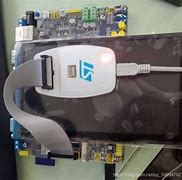
\includegraphics[scale = 0.7]{10}
	\caption{开发板与电脑相连}
\end{figure}

2.打开Keil软件界面,运行源程序代码,程序运行界面如图。
\begin{figure}[H]
	\centering
	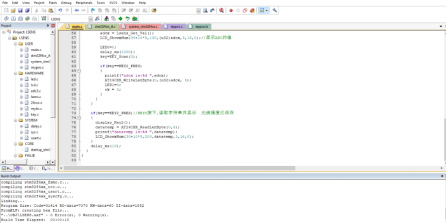
\includegraphics[scale = 0.7]{11}
	\caption{源程序运行界面}
\end{figure}

3.通过JTAK接口向STM32F4主芯片烧程序,关键烧入顺序过程如图。
\begin{figure}[H]
	\centering
	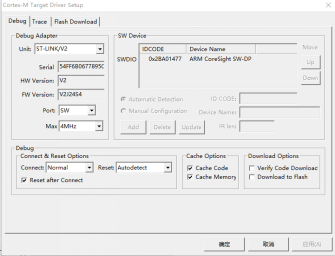
\includegraphics[scale = 0.7]{12}
\end{figure}
\begin{figure}[H]
	\centering
	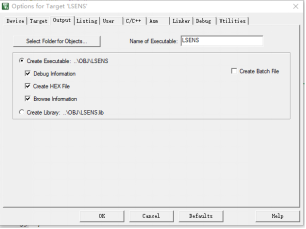
\includegraphics[scale = 0.7]{13}
\end{figure}
\begin{figure}[H]
	\centering
	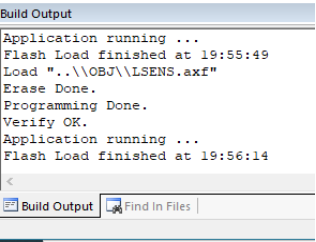
\includegraphics[scale = 0.7]{14}
\end{figure}

4.观察显示屏上的数据显示,将程序烧入STM32芯片后,显示屏的显示结果如图所示。在进行手写字体输入后在屏幕上可显示程序所识别到的字体的可能性。
\begin{figure}[H]
	\centering
	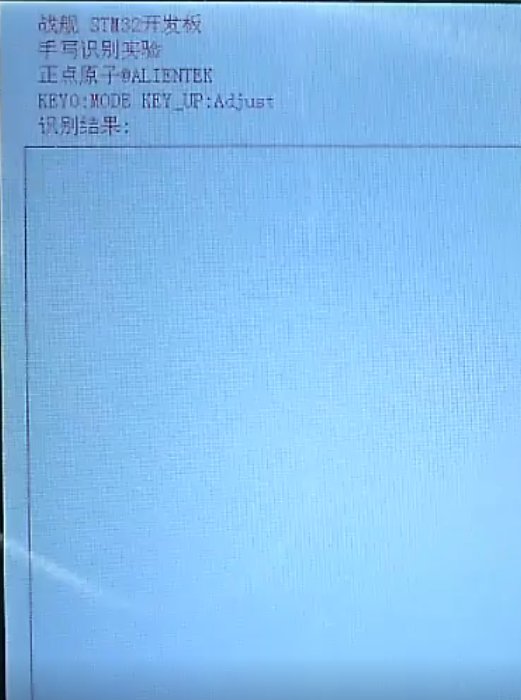
\includegraphics[scale = 0.3]{15}
\end{figure}
\begin{figure}[H]
	\centering
	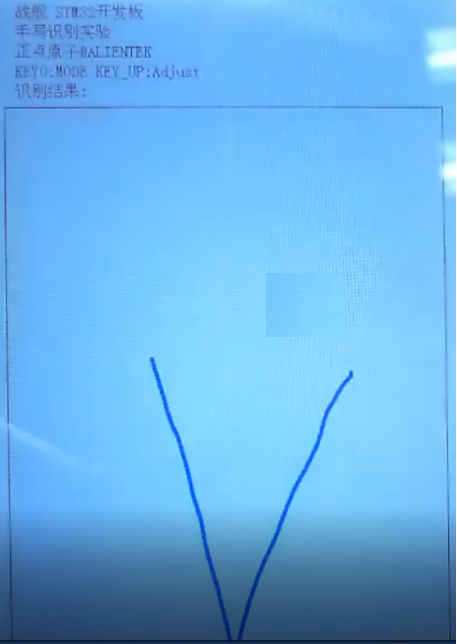
\includegraphics[scale = 0.3]{16}
\end{figure}
\begin{figure}[H]
	\centering
	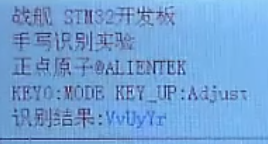
\includegraphics[scale = 0.3]{17}
\end{figure}

\section{项目设计总结}
本设计课题基于STM32F4单片机微控制器的实时数字设别系统,目的是通过采集屏幕上输入的笔画,从而进行输入的数字进行预测。手写识别,是指对在手写设备上书写时产生的有序轨迹信息进行识别的过程,是人际交互最自然、最方便的手段之一。随着智能手机和平板电脑等移动设备的普及,手写识别的应用也被越来越多的设备采用。手写识别能够使用户按照最自然、最方便的输入方式进行文字输入,易学易用,可取代键盘或者鼠标。用于手写输入的设备有许多种,比如电磁感应手写板、压感式手写板、触摸屏、触控板、超声波笔等。整个系统更加有趣,更加智能化、人性化。从产品研究与开发的角度思考,现对以后的进一步研究提出以下建议:产品整体的外形可以进行更进一步的优化,使之看起来更加美观,在使用的同时也可以增加它的观赏性,从而获得更多人的认可和青眯,使本设计能批量投入生产,真正发挥它的作用。并且产品本身在软件功能上还可以进一步优化,使系统本身符合工业需求。
\end{document}